\documentclass[a4paper,12pt]{article}

\usepackage{../header}
\newcommand{\school}{ntu}
\newcommand{\subject}{math}
\renewcommand{\year}{104}
\newcommand{\titlename}{\MakeUppercase{\school} \subject \ \year}

\fancypagestyle{mainmatter}{\rhead{\titlename}}
\pagestyle{mainmatter}
\CenterWallPaper{.50}{img/logo_ntu_recolor.jpg}
\newcommand{\ver}{\textsc{Version} 1.0} % Version number.

\begin{document}

\title{\LARGE{\textbf{Solutions}} \\
	\Huge{\textbf{\titlename}} \\
	\normalsize{\ver}
}
\author{}
\date{}

\maketitle

% Start of solutions.

\begin{enumerate}
	\item We have \begin{equation}
		\begin{aligned}
			& p \rightarrow q \\
			\iff & \ \neg p \lor q
		\end{aligned}
	\end{equation}
	\begin{enumerate}[label=(\alph*)]
		\item True.
		\item False, since \begin{equation}
			\begin{aligned}
				& \neg p \rightarrow \neg q \\
				\iff & \ p \lor \neg q \neq \neg p \lor q
			\end{aligned}
		\end{equation}
		\item False, since \begin{equation}
			\begin{aligned}
				& q \rightarrow p \\
				\iff & \ \neg q \lor p \neq \neg p \lor q
			\end{aligned}
		\end{equation}
		\item True, since \begin{equation}
			\begin{aligned}
				& \neg q \rightarrow \neg p \\
				\iff & \ q \lor \neg p = \neg p \lor q
			\end{aligned}
		\end{equation}
		\item False, since \begin{equation}
			\begin{aligned}
				& \neg q \rightarrow p \\
				\iff & \ q \lor p \neq \neg p \lor q
			\end{aligned}
		\end{equation}
	\end{enumerate}
	\begin{answer}{$\dag$}\begin{equation}
			ad
		\end{equation}
	\end{answer}
	\item We have \quad\begin{figure}[H]
		\centering
		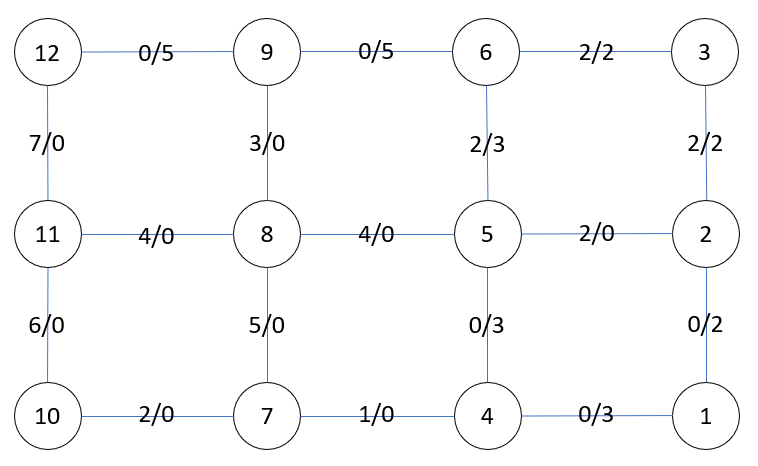
\includegraphics[scale=0.6]{img/ntu_104_math_2.png}
		\label{img:ntu_104_math_2}
	\end{figure}
	\begin{answer}{$\dag$}\begin{equation}
			5	
		\end{equation}
	\end{answer}
	\item We have \begin{equation}
		(1 + x)^n = \sum_{i = 0}^{n}\binom{n}{i}x^n
	\end{equation}
	\begin{answer}{$\dag$}\begin{equation}
			3^n
		\end{equation}
	\end{answer}
	\item We have \begin{equation}
		120 = 2^3 \times 3^1 \times 5^1
	\end{equation}
	\begin{answer}{$\dag$}\begin{equation}
			\Phi(120) = 120 \times \frac{1}{2} \times \frac{2}{3} \times \frac{4}{5} = 32
		\end{equation}
	\end{answer}
	\item Suppose \begin{equation}
		\begin{aligned}
			y_1 & = x_1 - 1 \\
			y_2 & = x_2 - x_1 \\
			y_3 & = x_3 - x_2 \\
			& \ \ \vdots \\
			y_n & = x_n - x_{n - 1} \\
			y_{n + 1} & = r - x_n
		\end{aligned}
	\end{equation} We have \begin{equation}
		\begin{aligned}
			& \begin{cases}
				y_i \ge 1, \ \forall \ 1 \le i \le n \\
				x_1 \ge 1, \ x_2 \ge 2, \ \cdots, \ x_{n - 1} \ge (n - 1)
			\end{cases} \\
			\Rightarrow & \ y_{n + 1} = r - x_n = x_1 + x_2 + \cdots + x_{n - 1} \ge \frac{n(n - 1)}{2}
		\end{aligned}
	\end{equation} Then, we have \begin{equation}
		\begin{aligned}
			& y_1 + 2 \times y_2 + \cdots + n \times y_n + (n + 1) \times y_{n + 1} \\
			= & \ (x_1 - 1) + 2 \times (x_2 - x_1) + 3 \times (x_3 - x_2) + \cdots + n \times (x_n - x_{n - 1}) \\
			+ & \ (n + 1) \times (r - x_n) \\
			= & \ -1 - x_1 - x_2 - x_3 - \cdots - x_n + (n + 1) \times r \\
			= & \ nr - 1
		\end{aligned}
	\end{equation} Then, we have new generating function \begin{equation}
		\begin{aligned}
			G(x) = & (1 + x + x^2 + \cdots)(x^2 + x^4 + x^6 + \cdots)(x^3 + x^6 + x^9 + \cdots)\cdots \\
			& (x^n + x^{2n} + x^{3n} + \cdots)(x^{(n + 1)\frac{n(n - 1)}{2}} + \cdots) \\
			= & \frac{1}{1 - x}\frac{x^2}{1 - x^2}\frac{x^3}{1 - x^3}\cdots\frac{x^n}{1 - x^n}\frac{x^{\frac{(n^2 - 1)}{2}}}{1 - x^{n + 1}}
		\end{aligned}
	\end{equation}
	\begin{answer}{$\dag$} Coefficient of $x^{nr - 1}$ of \begin{equation}
		\frac{1}{1 - x}\frac{x^2}{1 - x^2}\frac{x^3}{1 - x^3}\cdots\frac{x^n}{1 - x^n}\frac{x^{\frac{(n^2 - 1)}{2}}}{1 - x^{n + 1}}
		\end{equation}
	\end{answer}
	\item We have \begin{equation}
		\begin{aligned}
			\Rightarrow & \ \alpha = 2 \\
			\Rightarrow & \ \begin{cases}
				a_n^{(h)} = c \times 2^n \\
				a_n^{(p)} = d \times 3^n
			\end{cases}
		\end{aligned}
	\end{equation} Then, we have \begin{equation}
		\begin{aligned}
			& d \times 3^n = 2 \times d \times 3^{n - 1} + 3^{n - 1} \\
			\Rightarrow & \ d = 1 \\
			\Rightarrow & \ a_n = c \times 2^n + 3^n
		\end{aligned}
	\end{equation} Then, we have \begin{equation}
		\begin{aligned}
			& a_0 = 2 = c + 1 \\
			\Rightarrow & \ c = 1
		\end{aligned}
	\end{equation}
	\begin{answer}{$\dag$}\begin{equation}
			a_n = 2^n + 3^n
		\end{equation}
	\end{answer}
	\item We have \begin{equation}
		\tr(\mat{XY}) = \tr((\mat{XY})\herm) = \tr(\mat{Y}\herm\mat{X}\herm) = \tr(\overline{\mat{Y}^\intercal\mat{X}^\intercal}) = \tr(\overline{(\mat{XY})^\intercal}) = \tr(\overline{\mat{XY}})
	\end{equation}
	\begin{answer}{$\dag$}\begin{equation}
			a
		\end{equation}
	\end{answer}
	\item We have \begin{equation}
		\mat{A} \overset{\text{rref}}= \begin{bmatrix}
			0 & 1 & 2 & 1 & 1 \\
			0 & 0 & 0 & 0 & 0 \\
			1 & 0 & -1 & 2 & 1 \\
			0 & 0 & 0 & 2 & 4
		\end{bmatrix}
	\end{equation} We have $\rnk{\mat{A}} = 3$. Then, we have \begin{equation}
		\begin{aligned}
			& \rnk(\mat{A}) + \rnk(\mat{B}) - 5 \le \rnk(\mat{AB}) \\
			\Rightarrow & \ 3 + \rnk(\mat{B}) - 5 \le 0 \\
		\end{aligned}
	\end{equation}
	\begin{answer}{$\dag$}\begin{equation}
			\rnk(\mat{B}) \le 2
		\end{equation}
	\end{answer}
	\item \begin{answer}{$\dag$} Sum of eigenvalues equals to the trace. \begin{equation}
			2 + 2 + 2 + 2 = 8
		\end{equation}
	\end{answer}
	\item \begin{answer}{$\dag$} The problem is \textbf{WRONG}, since $\{\mat{A}_1, \ \mat{A}_2, \ \mat{A}_3, \ \mat{B}_1\}$ is linearly independent.
	\end{answer}
	\item We have \begin{equation}
		[f]_{\beta} = \begin{bmatrix}
			f(\beta_1, \beta_1) & f(\beta_2, \beta_1) & f(\beta_3, \beta_1) & f(\beta_4, \beta_1) \\
			f(\beta_1, \beta_2) & f(\beta_2, \beta_2) & f(\beta_3, \beta_2) & f(\beta_4, \beta_2) \\
			f(\beta_1, \beta_3) & f(\beta_2, \beta_3) & f(\beta_3, \beta_3) & f(\beta_4, \beta_3) \\
			f(\beta_1, \beta_4) & f(\beta_2, \beta_4) & f(\beta_3, \beta_4) & f(\beta_4, \beta_4)
		\end{bmatrix}
	\end{equation}
	\begin{answer}{$\dag$}\begin{equation}
			[f]_{\beta} = \begin{bmatrix}
				1 & 0 & 0 & 1 \\
				0 & 0 & 0 & 0 \\
				0 & 0 & 0 & 0 \\
				1 & 0 & 0 & 1
			\end{bmatrix}
		\end{equation}
	\end{answer}
\end{enumerate}

% End of solutions.

\end{document}
